\chapter{Regression}
\section{Model Based Regression}
In this section we will study model-based regression, which means the models of the data and the error are given and we are only interested in finding the \textit{regression function}, also called \textit{optimal estimator}.

Suppose we have $Y \in \mathbb{R}$ (that is our parameter of interest) and data $X \in \mathbb{R}^d$, both random variables.

\begin{definition}
    The optimal regression function is the mean of the posterior distribution of the target variable given the data, i.e. the \textbf{MMSE}:
    \[
        r(X) = \E{}{Y\mid X}
    \]
\end{definition}

\begin{exercise}
    Compute the regression function for the multiple linear regression model:
    \[
        Y = \beta_0 + \sum_{i=1}^{d} \beta_i X_i + \mathcal{E}
    \]
    where $Y$ is the response variable, $\beta_0$ is the intercept term, $\beta_i$ are the coefficients of the regressors $X_i$ and $\mathcal{E}$ is the error term.

    The common assumption we do in multiple linear regression is that $\mathcal{E}$ is a zero mean random variable with variance $\sigma^2$.

    Let us rewrite the model in matrix form:
    \[
        Y   = \beta^T X + \mathcal{E}
    \]
    where $\beta = (\beta_0, \beta_1, \dots, \beta_d)^T$ is the \textit{parameters} vector and $X = (1, X_1, \dots, X_d)^T$ is the \textit{predictors} vector.\footnote{We can write this both as $\beta^T X$ or $X^T \beta$ because the final product is a scalar thus the order of the product doesn't matter, but we will use the first notation.}

    Now we can compute the regression function:
    \[
        r(X) = \E{}{Y \mid X} = \E{}{\beta^T X + \mathcal{E} \mid X}
    \]
    By applying the linearity properties of the expectation:
    \[
        r(X) = \beta^T \E{}{X \mid X}  + \E{}{\mathcal{E} \mid X}
    \]
    The first expectation $\E{}{X \mid X}$ is $X$ because we are conditioning on $X$ and $X$ is a constant given $X$, while the second expectation $\E{}{\mathcal{E} \mid X}$ is zero because in this setting we need to assume that $\mathcal{E}$ is conditionally zero mean given $X$.

    In conclusion, we found that the optimal regression function for the multiple linear regression model is:
    \[
        r(X) = \beta^T X
    \]

\end{exercise}
\begin{theorem}
    Assuming a general regression problem, i.e. $Y_0 = r(X_0) + \mathcal{E}$, the error is conditionally zero mean:
    \[
        \E{}{\mathcal{E} \mid X} = 0
    \]
\end{theorem}

\begin{proof}
    The error is defined as following:
    \[
        \mathcal{E} = Y_0 - r(X_0)
    \]
    We can compute the conditional expectation of the error given $X$:
    \[
        \E{}{\mathcal{E} \mid X_0} = \E{}{Y_0 - r(X_0) \mid X_0} = \E{}{Y_0 \mid X_0} - r(X_0)
    \]
    The first term is the conditional expectation of $Y_0$ given $X_0$, which is equal to $r(X_0)$ by definition of regression function. So we get the following:
    \[
        \E{}{\mathcal{E} \mid X_0} = r(X_0) - r(X_0) = 0
    \]
\end{proof}

Note that if we assumed the shape of optimal function, like we did in the linear regression case, we need to make the assumption that the error is conditionally zero mean. If this assumption wasn't true, it would mean that we made a wrong assumption on the shape of the optimal function.
\[
    \E{}{\mathcal{E} \mid X_0} = r(X_0) - \beta^T X_0 \neq 0 \implies r(X_0) \neq \beta^T X_0
\]

\begin{exercise}
    Find the relationship between $\beta$ and $X$ and $Y$. In particular, we want to find an expression for $\beta$ that depends on some moments of $X,Y$ and $XY$.

    Assume we are working with the multiple linear regression model:
    \[
        Y = X^T \beta + \mathcal{E}
    \]
    where $Y \in \mathbb{R}$, $X \in \mathbb{R}^{(d+1) \times 1}$, $\beta \in \mathbb{R}^{(d+1) \times 1}$ and $\mathcal{E} \in \mathbb{R}$.

    First, since tipically the vector relation $a^Tb$ is not invertible, we multiply on the left both members by $X$ in order to create a matricial relation:
    \[
        \underset{(d+1) \times 1}{XY} = \underset{(d+1)\times 1}{X X^T\beta} + \underset{(d+1)\times 1}{X\mathcal{E}}
    \]
    Then we take expectation, to remove the unknown error term, and we get the following relation:
    \begin{equation}
        \E{}{XY} = \E{}{X X^T} \beta + \E{}{X \varepsilon} \label{eq:1}
    \end{equation}
    And we compute each term separately.

    For the first term, we can observe that the parameter vector is a constant with respect to $X$ so we can take it out of the expectation. To compute the expectation of the matrix $X^T X$, let's consider a generic entry:
    \[
        [X X^T]_{ij} = X_i X_j \to \E{}{[X X^T]_{ij}} = \E{}{X_i X_j}
    \]
    Since the expected value between $X_i X_j$ is a correlation, $XX^T$ is a quantity that describes the correlation between the data.
    \begin{definition}
        The matrix $R_X \triangleq \E{}{X X^T}$ is the \textbf{(auto)-correlation matrix}.
    \end{definition}
    The same reasoning can be applied to $\E{}{XY}$, where we get a corretlation between the data and the response variabile.
    \begin{definition}
        The matrix $R_{XY} \triangleq \E{}{X Y}$ is the \textbf{(cross)-correlation matrix}.
    \end{definition}

    As for the second term, since $X$ and $\mathcal{E}$ are not independent, we apply the tower property:
    \[
        \E{}{X \mathcal{E}} = \E{X}{\E{}{X \mathcal{E} | X}} = \E{X}{X \E{}{\mathcal{E} | X}} = 0
    \]
    since in the inner expectation $X$ is a constant, it can be taken out of the expectation and since we assumed that the error term is zero mean given $X$, we find out that the whole expectation is zero.

    We can rewrite the equation \ref{eq:1} as:
    \[
        R_{XY} =  R_X \beta
    \]
    And then solve for $\beta$:\footnote{By assuming that $R_x$ is invertible.}
    \[
        \beta = R_X^{-1} R_{XY}
    \]
    Finding a new expression for the optimal regression function:
    \[
        r(X) = X^T\beta = X^TR_X^{-1}R_{XY}
    \]
    In conclusion we found out that in a model-based linear regression problem $\beta$ cannot be arbitrary, because it is uniquely determined by the correlation matrices of $X$ and $XY$.
\end{exercise}

\subsection{Connection between model-based and supervised}
\textbf{\textit{What is changing with respect to the other part of the course?}}

In the other part of the course we've worked in a \textbf{supervised} setting, meaning that we had a training set. We still had a model because we \textit{assumed} that the relationship between $Y$ and $X$ was linear, but we wanted to learn the parameters $\beta$ of the model from the data, making it a \textit{parametric regression} problem.

Recall that the prediction phase it's our most important goal and it is the goal we would have if we knew the model. Since we don't have the model, in the \textit{parametric} setting, we need to assume a model and learn the parameters $\beta$. In that case, learning $\beta$ is instrumental to \textit{predict} $Y$.

In our case, we are in a model-based setting, which means we do not have a training set. As we showed in the previous exercise, in our case, the parameters $\beta$ are not to be learned from the data, but they are uniquely determined by the correlation matrices of $X$ and $XY$.

% Sentire registrazione
% If we need information about $\beta$ we are solving inference\dots
% This (regression) is the simplest example of \textbf{MMSE} estimator.
% In practice we assume there is linear relationship and we don't have information about data, e.g. correlation matrix.

%\paragraph*{Clarification}
%When we have an estimation problem, we have our data and our goal is estimate %$Y$ from $X$. If we have one model we have one "theory", e.g. bayesian theory. In estimation, the MMSE is the optimal way to solve the problem.
%
%We have one model but this model is not perfectly known. We try to learn the %model, because our purpose is \textit{still} to estimate $Y$.
%
%In one case we have a \textbf{perfectly known model}, then we can use MMSE %theory, and we can compute the MMSE since we know the model and the distributions. In the other case we have a \textbf{model} but you don't know it perfectly. Then we have to \textbf{learn} the model. Then we need to learn %$\beta$. Note that the goal is still to estimate $Y$.

Now the question is \textbf{\textit{how can we learn the model}}?

In a supervised approach we use a \textbf{training set} $\tilde{X}$ (not a \textit{dataset}).
\[
    \tilde X=
    \begin{bmatrix}
        \tilde X_{11}     & \dots  & \tilde X_{1n}     \\
        \vdots            & \ddots & \vdots            \\
        \tilde X_{(d+1)1} & \dots  & \tilde X_{(d+1)n}
    \end{bmatrix}\\
\]
That we can write compactly as:
\[
    \tilde{X} = \left[
        \tilde{X}_1, \tilde{X}_2, \dots, \tilde{X}_n
        \right]
\]
Where each $\tilde{X}$ is a vector with dimensions $(d+1) \times 1$.

And the corrisponding values of the response variable, $\tilde{Y}$:
\[
    \tilde{Y} =   \left[
        \tilde{Y}_1, \tilde{Y}_2, \dots, \tilde{Y}_n
        \right]
\]
\begin{exercise}
    Propose an estimator $\hat{\beta}$ based on the training set $(\tilde{X}, \tilde{Y})$, knowing that $\beta = R_x^{-1} R_{xy}$ and $Y = \beta^T X$.

    We can find the estimator by replacing the correlation matrices with their empirical counterparts:
    \[
        \hat{\beta} = \left(\hat{R}_X\right)^{-1} \hat{R}_{XY}
    \]
    where the correlation matrices are defined as:
    \[
        [\hat{R}_{X}]_{ij} = \frac{1}{n} \sum_{m=1}^{n} \tilde{X}_{im} \tilde{X}_{mj}
        \qquad
        [\hat{R}_{XY}]_i = \frac{1}{n} \sum_{m=1}^{n} \tilde{X}_{im} \tilde{Y}_{m}
    \]
    % note that component $i$ is the row while component $j$ is the column.
    We can rewrite the estimators by using the matrix notation:
    \[
        [\hat{R}_{X}]_{ij} = \frac{1}{n} \left[\tilde{X}\tilde{X}^T\right]_{ij}
        \qquad
        [\hat{R}_{XY}]_i = \frac{1}{n} \left[\tilde{X} \tilde{Y}^T\right]_i
    \]
    By replacing the correlation matrices in the estimator and simplyfing $n$ we get:
    \[
        \hat{\beta} = \left(\hat{R}_X\right)^{-1} \hat{R}_{XY} = \left(\tilde{X} \tilde{X}^T\right)^{-1}  \tilde{X} \tilde{Y}^T
    \]

    The \textbf{empirical estimator} of $\beta$ we found is the same as the one we obtained in the supervised approach. In that case, we minimized the RSS, which, if divided by $n$, is the empirical risk.
    \[
        RSS = \frac{1}{n} \sum_{m=1}^{n} \left(\tilde{Y}_m - \beta^T \tilde{X}_m \right)^2 \xrightarrow{n \to +\infty} \E{}{(Y - \beta^T X)^2}
    \]
\end{exercise}
%TODO: non ho capito miriam cosa voleva dire qui, riporto le note nei miei appunti e poi ne discutiamo
% \begin{note}{Warning}
%     Sentire la registrazione da qui in poi.
% \end{note}

% The two things are connected only in this case.

% We took the optimal risk (that is the expectation) and we replaced it with the empirical risk. I am trying to do Bayes empirically. The difference is that we need a model. In MMSE we have a \textbf{general solution} that works for every model, in the \textbf{supervised approach} we need to impose or assume a model.

% Optimal Bayes is a benchmark performance. There is some optimal thing to do, we cannot do it. I impose one model and replace the \textit{optimal risk} with the \textit{empirical risk}.
Let's analyze what happened. We fall in a supervised learning problem, where we imposed a shape for the model and we want to learn $\beta$ in order to predict $Y$. There are roughly two possible ways:
\begin{enumerate}
    \item Try to emulate the shape of the optimal $\beta$ by estimating the matrices (correlation and cross-correlation) and then compute the estimator $\hat{\beta}$.
    \item Try to find the best $\beta$ that minimizes the empirical risk. Simply, we try to apply Bayes theory empirically.
\end{enumerate}
In this case, both approaches lead to the same result and are connected from the fact that both are linked to Bayes theory.

\subsection{Benchmark performance}

Both in the model-based and supervised case, the final goal is to make a prediction.

In model-based regression we want to find the expression of $Y$ which allows us to compute $Y$ knowing the distribution of $X$ and the parameters. In supervised regression, we want to make a prediction by exploiting the information contained inside the training set pairs, which must reveal the link between $X$ and $Y$.

Assume we have a training set $T_n = \{(X_i, Y_i)\}_{i=1}^n$, i.e. a set of examples of the link between the data $X$ and the response $Y$, and we want to make a prediction for a new observation $(X_0, Y_0)$. Making a prediction means that we want to predict $Y_0$, that is not observed, given the observation $X_0$. It is important to remark that we are working under the assumption that $X_0$ and $Y_0$ share the same distribution of $X_i$ and $Y_i$ but are outside $T_n$ in order to make it independent by $T_n$!.

In the model-based approach, the optimal estimator is the regression function $r(X_0)$, which is given by the MMSE. In the supervised approach, the estimator is the regression function $\hat{r}(X_0)$, which is given by the minimization of the empirical risk. This function will be a \textbf{suboptimal} estimator, meaning that it will not reach the performance of the MMSE.

\begin{theorem}\label{thm:1}
    The error of the suboptimal regression function $\hat{r}(X_0)$ is given by:
    \[
        \E{}{(\hat{r}(X_0) - Y_0)^2} = \text{MMSE} + \E{}{\left(\hat{r}(X_0) - r(X_0)\right)}
    \]
    where $\text{MMSE} = \E{}{(r(X_0) - Y_0)^2}$ is the error of the optimal estimator.
\end{theorem}

To prove this result, we first need to introduce the \textbf{orthogonality principle}.
\begin{theorem}
    The \textbf{orthogonality principle}, also called \textbf{Fundamental Result of MMSE}, states that the error of the optimal estimator is orthogonal to any (integrable) function of the data $g(X_0)$:
    \[
        \E{}{g(X_0) \left[ r(X_0) - Y_0\right]} = 0\quad \forall g(X_0)
    \]
\end{theorem}

\begin{proof}
    To prove the theorem \ref*{thm:1}, we need to compare the error of the suboptimal estimator with the error of the optimal estimator. The error of $\hat{r}(X_0)$ is given by:
    \[
        \E{}{(\hat{r}(X_0) - Y_0)^2}
    \]
    In order to compare it with the optimal estimator, we need to introduce the term of comparison inside the equation, by adding and subtracting $r(X_0)$ from the error term:
    \[
        \E{}{(\hat{r}(X_0) - Y_0)^2} =  \E{}{(\hat{r}(X_0) - r(X_0) + r(X_0) - Y_0)^2}
    \]
    Let's managing it as a square of binomial:
    \[
        \E{}{(\hat{r}(X_0) - Y_0)^2} =  \E{}{([\hat{r}(X_0) - r(X_0)] + [r(X_0) - Y_0])^2}
    \]
    By expanding the square we get:
    \[
        \E{}{([\hat{r}(X_0) - r(X_0)]^2 + [r(X_0) - Y_0]^2 + 2 [\hat{r}(X_0) - r(X_0)][r(X_0) - Y_0])}
    \]
    And applying the linearity property:
    \[
        \E{}{[\hat{r}(X_0) - r(X_0)]^2 }+ \E{}{[r(X_0) - Y_0]^2} + 2 \E{}{[\hat{r}(X_0) - r(X_0)][r(X_0) - Y_0]}
    \]
    The first term quantifies how much our regression function is deviated from the optimal regression function, the second term is the MMSE, the third term need further discussion.

    Since in the expectation there are two random variables $X_0$ and $Y_0$ and they are dependent, we cannot split the expectation. In order to get $X_0$ fixed, we would need to have a conditional expectation.

    We apply the \textit{tower property} on the third term:

    \begin{align*}
        \E{}{[\hat{r}(X_0) - r(X_0)][r(X_0) - Y_0]} = \E{X_0} {\E{Y_0}{\underbrace{[\hat{r}(X_0) - r(X_0)]}_{g(X_0)}[r(X_0)-Y_0]  \mid X_0}} = \\
        = \E{X_0} {g(X_0)\E{Y_0}{r(X_0)-Y_0 \mid X_0}} = \\
        = \E{X_0} {g(X_0)\{\E{Y_0}{r(X_0)\mid X_0}-\underbrace{\E{Y_0}{Y_0 \mid X_0}}_{r(X_0)}\}} = \\
        = \E{X_0}{ \E{Y_0}{g(X_0) \left(r(X_0) - r(X_0)\right)}} = 0                                         \\
    \end{align*}

    The last equality is true because of the \textbf{orthogonality principle}.

    So we can rewrite the error of the $\hat{r}(X_0)$ as:
    \[
        \boxed{
            \E{}{(\hat{r}(X_0) - Y_0)^2} = \text{MMSE} + \E{}{\left(\hat{r}(X_0) - r(X_0)\right)}}
    \]
\end{proof}

In conclusion, we can say that the error of the suboptimal estimator is the sum of the error of the optimal estimator and a \textbf{penalty term}, which is the squared difference between the arbitrary function and the optimal estimator. If our arbitrary function is the optimal estimator, the penalty term is zero, but if it differs, the penalty term increases.

This result has been very useful to discover \textit{non-parametric approaches}. Before this result the non-parametric approaches tried to approximate the optimal regression function, but now we can try to find an arbitrary function that minimizes the penalty term. The only problem is that we don't know the optimal regression function, so we cannot compute easily the penalty term. As for the MMSE, it can be approximated by simulation.

\section{Supervised Parametric Regression}
\subsection{Simple Linear Regression}
In order to introduce the concept of \textit{supervised parametric regression}, we will start with the simplest case, the \textit{simple linear regression} on which we assume a linear relationship between the response variable and the predictor variable with the following model:
% Let's consider a simple linear regression model:
\[
    Y = \beta_0 + \beta_1 X + \varepsilon
\]
Where we make the \textbf{zero-mean error assumption}, so $\E{}{\varepsilon} = 0$. 

Assume we want to estimate the parameters $\beta_0$ and $\beta_1$ and find the estimated model:
\[
    \hat{Y} = \hat{\beta}_0 + \hat{\beta}_1 X
\]

Suppose we have a training set $\mathcal{D}_{tr} = \{(x_i, y_i)\}_{i=1}^n$. We can write:
\[
    \hat{Y}_i = \hat{\beta}_0 + \hat{\beta}_1 X_i \qquad i = 1,\dots, n
\]

\paragraph*{Ordinary Least Squares}
The Ordinary Least Squares method let us estimate the parameters $\hat{\beta}_0$, $\hat{\beta}_1$ by minimizing the residual sum of squares, which is defined as following:
\[
    \text{RSS}(\beta_0, \beta_1) = \sum_{i=1}^{n} e_i^2 = \sum_{i=1}^{n} (y_i - \hat{y}_i)^2 = \sum_{i=1}^{n} (y_i - \hat{\beta}_0 - \hat{\beta}_1 x_i)^2
\]
Where $e_i$ represents the difference between the observed value and the predicted value, also called \textit{residual}.

Under the assumption that the error term $\underline{\varepsilon} = (\varepsilon_1, \dots, \varepsilon_n)^T$:
\begin{itemize}
    \item $\E{}{\varepsilon_i} = 0, \forall i$
    \item $\var{\underline{\varepsilon}} = \sigma^2 I_n$ (\textbf{homoscedasticity})
\end{itemize}

The \textbf{least square estimates} of the parameters are:
\[
    \underline{\beta}^T = \left(\hat{\beta}_0, \hat{\beta}_1\right) = \arg\min_{(\beta_0, \beta_1)} \sum_{i=1}^{n} (y_i - \beta_0 - \beta_1 x_i)^2
\]

If the error terms are independent and identically distributed as normals $\varepsilon_i \sim N(0, \sigma^2)$, then the \textit{least squares estimates} are equal to the ones we obtain by \textit{maximum likelihood estimation}.

\paragraph*{Estimating parameters in simple linear regression}

Now we want to find the least squares estimates for the parameters $\hat{\beta}_0$ and $\hat{\beta}_1$. In order to solve the minimization problem, we need to compute the gradient with respect to the parameters $\underline{\beta}$ and set it to zero:
\[
    \nabla_{\underline{\beta}} RSS(\beta_0, \beta_1) = 0
\]

\[
    \begin{cases}
        \frac{\partial RSS}{\partial \beta_0} = -2 \sum_{i=1}^{n} (y_i - \beta_0 - \beta_1 x_i) = 0 \\
        \frac{\partial RSS}{\partial \beta_1} =   -2 \sum_{i=1}^{n} x_i (y_i - \beta_0 - \beta_1 x_i) = 0
    \end{cases}
\]

%TODO: Fare il controllo su punto di minimo con derivata seconda
\[
    \begin{cases}
        n\beta_0 + \beta_1 \sum_{i=1}^n x_i = \sum_{i=1}^{n} y_i \\
        \beta_0 \sum_{i=1}^n x_i + \beta_1 \sum_{i=1}^n x_i^2 = \sum_{i=1}^{n} x_i y_i
    \end{cases}
\]
Let's define the following quantities:
\[
    \overline{x} = \frac{1}{n} \sum_{i=1}^n x_i
    \qquad
    \overline{y} = \frac{1}{n} \sum_{i=1}^n y_i
\]
From the first equation we can find $\beta_0$:
\[
    \beta_0 = \overline{y} - \beta_1 \overline{x}
\]
Substituting this value into the second equation we can find $\beta_1$:
\[
    \overline{y} \sum_{i=1}^n x_i - \beta_1 \overline{x} \sum_{i=1}^n x_i + \beta_1 \sum_{i=1}^n x_i^2 = \sum_{i=1}^{n} x_i y_i \leftrightarrow \beta_1 = \frac{\sum_{i=1}^{n} x_i y_i - \overline{y} \sum_{i=1}^n x_i}{\sum_{i=1}^n x_i^2 - \overline{x} \sum_{i=1}^n x_i}
\]

The least squares estimates are the following:
\[
    \begin{cases}
        \hat{\beta}_0 = \overline{y} - \hat{\beta}_1 \overline{x} \\
        \hat{\beta}_1 = \frac{\sum_{i=1}^{n} (x_i - \overline{x})(y_i - \overline{y})}{\sum_{i=1}^n (x_i - \overline{x})^2}
    \end{cases}
\]

\callout{Note}{Some books indicates the previous with $B_0$ and $B_1$ because they have the meaning of \textit{estimators}. For notation simplicity, we will use $\hat{\beta}_0$ and $\hat{\beta}_1$.}
The \textbf{Gauss-Markov} theorem states that, in a model where the errors are zero-mean, incorrelated and homoschedastic, the least squares estimates are the \textbf{best linear unbiased estimates} (BLUE) of the parameters $\beta_0$ and $\beta_1$.

%NOTA: non mi trovo con quello che ha scritto Miriam, quello indicato è l'RSE ed è la stima della dev std di epsilon non di beta. INoltre i beta non hanno la stessa varianza
% This means that the least squares estimates are unbiased and have the \textit{same} smallest variance:
% \[
%     \sigma^2 = \text{RSE}^2 = \frac{\text{RSS}(\hat{\beta}_0, \hat{\beta}_1)}{n-2}
% \]
\[
    \E{}{\hat{\beta}_0} = \beta_0
    \qquad
    \E{}{\hat{\beta}_1} = \beta_1
\]

The \textbf{variance} of the estimates made using OLS is given by:
\[
    \text{SE}(\hat{\beta}_0)^2 = \sigma^2\left[\frac 1n + \frac{\bar x^2}{\sum_{i=1}^n(x_i-\bar x)^2}\right] 
    \qquad
    \text{SE}(\hat{\beta}_1)^2 = \frac{\sigma^2}{\sum_{i=1}^n(x_i-\bar x)^2}
\]

where $\sigma^2$ is the variance of the error term $\varepsilon$ and it is unknown. We can estimate it using the \textbf{residual standard error} under the homoschedasticity assumption:
\[
    \text{RSE} = \sqrt{\frac{1}{n-2} \sum_{i=1}^{n} (y_i - \hat{y}_i)^2} = \sqrt{\frac{1}{n-2} \text{RSS}}
\]

At the denominator of the RSE there is, in general case, $n-p-1$ where $p$ is the number of predictors. In the simple linear regression case, $p=1$ and the denominator is $n-2$. It is also known as the \textbf{degrees of freedom} of the model.

\subparagraph*{Confidence intervals}
The \textbf{confidence intervals} tells us the interval on which, after repeating an estimation experiment many times, we would expect the true value of the parameter to fall given a certaing \textbf{confidence level} or \textbf{error level}.
\callout{Note}{The \textit{error level} is mandatory since, otherwise, the intervall should be from $-\infty$ to $+\infty$.}
The assumptions to make about the errors $\varepsilon_i$ are the following:
\begin{itemize}
    \item \textbf{Homoschedasticity}: the errors $\varepsilon_i$ have the same variance
    \item \textbf{Independence}: the errors $\varepsilon_i$ are independent
    \item \textbf{Normality}: the errors $\varepsilon_i$ are normally distributed.\footnote{This assumption is not necessary to compute the least squares estimates, but it is necessary to compute the confidence intervals.}
\end{itemize}
% By assuming that the errors $\varepsilon_i$ are normally distributed, we can compute the confidence intervals for the parameters $\beta_0$ and $\beta_1$:
It's useful to compute that intervals for $\beta_0$ and $\beta_1$. 
Let's call $B_0$ and $B_1$ the random variables that represent the estimates of $\beta_0$ and $\beta_1$ respectively. Since we know the distribution of the errors $\varepsilon_i$, we can compute the distribution of $B_0$ and $B_1$:
\[
    B_0 \sim N(\beta_0, SE^2(B_0))
\]
\[
    B_1 \sim N(\beta_1, SE^2(B_1))
\]

The following quantity:
\[
    \frac{B_1 - \beta_1}{SE(B_1)} \sim t_{n-2}
\]
is called \textbf{t-statistic} and it is used to compute the confidence interval for $\beta_1$. Since it is the ratio between a standard normal distribution and the square root of the ratio between a chi-square distribution and a number of degree of freedom, It is distributed as a (Student) $t$-distribution with $n-2$ degrees of freedom. %TODO: si potrebbe spiegare molto meglio. Se vogliamo allungare possimao farlo
%TODO: si potrebbe aggiungere immagine

By fixing an error level $\alpha$, we can define the inverval by knowing that:
\[
    \Pr{-t_{1-\alpha/2, n-2} \leq \frac{B- \beta}{SE(B)} \leq t_{1-\alpha/2, n-2}} = 1 - \alpha
\]
where we have not specificied the subscript for generality.

Since we want to know the interval where we can find $\beta$, we can write:
\[
    \Pr[B+SE(B)\cdot t_{1-\alpha/2, n-2} \leq \beta \leq B+SE(B)\cdot t_{1-\alpha/2, n-2}] = 1 - \alpha
\]
Evalutaing the estimator $B$ we obtain $\hat \beta$ and we can compute the interval:
\[
    L = \hat \beta - SE(\hat \beta) \cdot t_{1-\alpha/2, n-2}
    \qquad
    U = \hat \beta + SE(\hat \beta) \cdot t_{1-\alpha/2, n-2}
\]
The true value of $\beta$ is expected to fall in the interval $[L, U]$ with a confidence level of $1-\alpha$.

\subsection{Hypothesis testing}
In the simple linear regression case, we would like to know if the predictor $X$ has a significant effect on the response $Y$. In order to do that, we can perform a \textbf{hypothesis test} on the parameter $\beta_1$.
If that coefficient is not significantly different from zero, then the predictor $X$ has no effect on the response $Y$.

The hypotesis test is made by the \textit{null hypothesis} $H_0$ and the \textit{alternative hypothesis} $H_1$:
\[\begin{cases}
    H_0: \beta_1 = \beta^\ast_1 \text{ There is no relationship}\\
    H_1: \beta_1 \neq \beta^\ast_1 \text{ There is a relationship}
\end{cases}\]
This kind of test is said to be \textbf{bilateral} since, if the null hypothesis is rejected, we can say that there is a relationship between $X$ and $Y$, but we cannot say if it is positive or negative.
As we've done for the confidence intervals, we have to accept an error level $\alpha$.

In order to perform the test we need a \textbf{test statistic}.
Let's suppose that we want to test if $\beta_1$ is equal to a certain value $\beta_1^\ast$ (in our case $\beta_1^\ast = 0$). We can define the following test statistic:
\[
    t = \frac{B_1 - \beta_1^\ast}{SE(B_1)}
\]
We can note that, if the null hypothesis is true, the test statistic is distributed as a $t$-distribution with $n-2$ degrees of freedom. 
We can use this information to decide if we can reject the null hypothesis or not. If the evaluated test statistic is far from zero, probably the true value of $\beta_1$ is different from zero and we can reject the null hypothesis. If the test statistic is close to zero, we cannot reject the null hypothesis.

To be able to choose between the hypothesis we need to impose a threshold. For this reason we introduced $\alpha$, also called \textbf{I type risk}:
\[
    \Pr{\text{Reject } H_0 \mid H_0 \text{ is true}} = \alpha
\]
%TODO: inserire un'immagine
$\alpha$ is the area under the tails of the $t$-distribution when the null hypothesis is true, this area is called \textbf{critical region}.

Since the decision we make can have a very different meaning if the distance from 0 is greater or smaller, we introduce a value that measure the strongness of the evidence against the null hypothesis. This value is called \textbf{p-value} and it is the probability of observing a value of the test statistic greater than the one observed, assuming that the null hypothesis is true. The more the p-value is small, the more the evidence against the null hypothesis is strong. Formally:
\[
    p = \Pr{|t| \geq |t'|    \mid H_0 \text{ is true}}
\]
We can sintetize the decision rule as following:
\begin{itemize}
    \item If $p \leq \alpha$ we reject the null hypothesis
    \item If $p > \alpha$ we cannot reject the null hypothesis
\end{itemize}
%─────────────────────── THIS SLIDE ──────────────────
\subsection{Assessing the accuracy of the model}
In order to understand if the inffered model is good enough, we should use an error metric. If we're working with a continuous target variable, we can use the \textit{RSE} or \textbf{residual standard error}. The residual standard error measures how much of the variability is not explained by our model.

However, the residual standard error has the limitation that it depends on scale by the order of $Y$. If $Y$ is a large number, then the \textit{RSE} will also be a large number.

This means that it is not always clear what constitutes a good RSE. An alternative measure of fit is the $\mathbf{R^2}$ \textbf{statistic}.

This statistic represents the proportion of variance explained and it is independent of the scale of $Y$. The definition of \textit{R-squared} is the following:
\[
    R^2 = \frac{TSS - RSS}{TSS} = 1 - \frac{RSS}{TSS}
\]
Where \textbf{TSS} is the \textit{total sum of squares} and it is defined as following:
\[
    TSS = \sum_{i=1}^{n} (y_i - \overline{y})^2
\]
This quantity measures the total variance in the response $Y$ and represents the amount of variability inherent in the response before the regression is performed. In contrast, RSS measures the amount of variability that is left unexplained after performing the regression.

The difference between this two quantities measures the amount of variability in the response that is explained or removed by performing the regression and $R^2$ measures the proportion of variability in $Y$ that can be explained using $X$.
When the $R^2$ statistic is close to $1$ it means that a large proportion of the variability in the response has been explained by the regression.
When the $R^2$ statistic is close to $0$ it means that the regression did not explain much of the variability in the response and this might occur because the linear model is wrong or the inherent error is high or both.

In the simple regression setting:
\[
    R^2 = r^2
\]
Where $r$ is the Pearson's correlation index between $X$ and $Y$:
\[
    r = \frac{\sum_{i=1}^{n} (x_i - \overline{x})(y_i - \overline{y})}{\sqrt{\sum_{i=1}^{n} (x_i - \overline{x})^2} \sqrt{\sum_{i=1}^{n} (y_i - \overline{y})^2}}
\]
The correlation index is a measure of the linear relationship between $X$ and $Y$. The $R^2$ statistic extends the concept of correlation between multiple predictors and the response.

\subsection{Multiple Linear Regression}
Suppose we have an input vector $X^T = (X_1, \dots, X_p)$ and we want to predict an output $Y$. The linear regression model that we can assume in this setting has the shape:
\[
    Y = f(X) + \varepsilon = \beta_0 + \sum_{j=1}^{p} \beta_j X_j + \varepsilon
\]

We can interpret the model as the following: $\beta_j$ is the average increase in $Y$ when $X_j$ increases by one unit holding all others constants.

Note that despite being called \textbf{linear regression}, $X_j$ can come from different sources, such as:
\begin{itemize}
    \item transformations of the input function, e.g. $\log$
    \item polynomial fit, e.g. $X_2 = X_1^2$
    \item dummy coding of the levels of qualitative inputs
    \item interaction between variables $X_3 = X_1 \cdot X_2$
\end{itemize}


\subsubsection*{Least squares estimates}
As we said, given the input vector $X^T = (X_1, \dots, X_p)$, if we want to predict an output $Y$, we need a regression model, for example:
\[
    Y = f(X) + \varepsilon
\]
That model, under a linear assumption, become:
\[
    Y = \beta_0 + \sum_{j=1}^{p} \beta_j X_j + \varepsilon
\]
Assuming a zero-mean error, we can make prediction using the following model:
\[
    \hat{Y} = \hat{\beta}_0 + \sum_{j=1}^{p} \hat{\beta}_j X_j
\]
To apply the OLS approach, it's convenient to reason in a matrix form. 
\begin{gather*}
    \underline{X} = (X_1, \dots, X_p)\text{ input vector} \\
    \underline{\hat\beta} = (\hat\beta_0, \hat\beta_1, \dots, \hat\beta_p)^T\text{ parameter estimates vector} \\
\end{gather*}

Given the training data $\mathcal{D}_{tr} = \{ (x_i, y_i) \}_{i=1}^n$
we pick $\underline{\hat\beta}$ as the vector that minimize the residual sum of squares.
\[
    \text{RSS}(\underline \beta) = \sum_{i=1}^{n} (y_i - f(x_i))^2 = \sum_{i=1}^{n} \left(y_i - \beta_0 - \sum_{j=1}^{p} \beta_j x_{ij}\right)^2
\]
We can write our linear regression model in matrix form:
\[
    \underline Y = 
    \overset{[n\times 1]}{
        \begin{pmatrix}
            y_1 \\ \vdots \\ y_n 
        \end{pmatrix}
        } =
    \overset{[n\times(p+1)]}{
        \begin{pmatrix}
            1 & x_{11} & x_{12} & \dots & x_{1p} \\
            1 & x_{21} & x_{22} & \dots & x_{2p} \\ \vdots \\ 1 & x_{n1} & x_{n2} & \dots & x_{np}
        \end{pmatrix}
        }
    \overset{[(p+1)\times 1]}{
            \begin{pmatrix}
                \beta_0 \\ \beta_1 \\ \vdots \\ \beta_p 
            \end{pmatrix}
            } +
    \overset{[n\times 1]}{
        \begin{pmatrix}
            \epsilon_1\\
            \vdots \\
            \epsilon_n
        \end{pmatrix}}= \underline{\underline{X}} \underline \beta + \underline \epsilon
\]

So the estimated response on the traning set will be:
\[
    \hat{Y} = \underline{\underline{X}} \underline{\hat{\beta}}
\]
Now we can rewrite also the formula of the \textit{RSS} in matrix form:
\[
    \text{RSS}(\underline{\beta})  = \sum_{i=1}^{n} \left(y_i - (\underline{\underline{X}} \underline{\beta})_i\right)^2 = (\underline{Y} - \underline{\underline{X}} \underline{\beta})^T(\underline{Y} - \underline{\underline{X}} \underline{\beta})
\]
Now we need to compute the gradient of the residual sum of squares with respect to the parameters. Let's recall first the following rules:
\begin{enumerate}
    \item $\nabla_x a^t x = \nabla_x x^T a =  a$
    \item $\nabla_x x^T A x = A^t x + A x$
\end{enumerate}
The gradient of the RSS will be (underline omitted for simplicity):
\begin{align*}
    \nabla_\beta \text{RSS} (\beta) & = \nabla_\beta \left((Y- X\beta)^T (Y-X\beta) \right) =                                 \\
                                    & = \nabla_\beta \left(Y^T Y - \underbrace{Y^T X\beta}_{(1\times 1)} - \underbrace{\beta^T X^T Y}_{(1\times 1)} + \beta^T X^T X \beta \right) = \\
                                    & = \nabla_\beta\left(Y^T Y - 2 \beta^T X^T Y + \beta^T X^T X \beta\right) =              \\
                                    & = -2 X^T Y + \underbrace{(X^T X)^T \beta + (X^T X)^T \beta}_{\text{Second rule of gradient}} 
                                    % =                                        \\
                                    % & = X^T Y + (X^T X)^T \beta = 0 \iff \hat{\beta} = (X^T X)^{-1} X^T Y
\end{align*}
We can set the gradient to zero and solve for $\beta$:
\begin{align*}
    -2 X^T Y + 2(X^T X)^T \beta = 0 \implies \\
    X^T Y - (X^T X)^T \beta = 0 \implies \\
    (X^T X)^T \beta = X^T Y \implies \\
    \beta = (X^T X)^{-1} X^T Y    
\end{align*}


The \textit{least squares estimation} of the parameters are
\[
    \hat{\underline\beta} = (\underline {\underline X}^T \underline{\underline X} )^{-1} \underline{\underline X}^T \underline Y
\]

Note that durning the computation we also found that:
\[
    X^T Y - (X^T X)^T \hat \beta = X^T\underbrace{(Y-X\hat{\beta})}_{\underline {e}} = 0 \Rightarrow e \perp X
\]
Namely, we found that the vector $\hat{\underline \beta}$ that minimizes RSS, is chosen in such a way that the residual vector $\underline e$ is \textbf{orthogonal} to the data matrix $\underline {\underline X}$ that represents the subspace on which our predictors move.

Finally, to confirm that this solution is actually a point of minimum, we need to check the \textbf{hessian matrix}, defined as following:
\[
    \underline {\underline H}_{RSS}^{(\underline\beta)} = \frac{\partial^2 RSS(\underline\beta)}{\partial \underline\beta \partial \underline\beta^T} = 2 \underline {\underline X}^T \underline {\underline X}
\]
It can be shown that $\underline {\underline H}_{RSS}^{(\underline\beta)} = 2 \underline {\underline X}^T \underline {\underline X}$ is an estimator of the \textbf{variance-covariance matrix} of the predictors (columns of $\underline {\underline X}$). By definition, this matrix is \textit{positive semidefinite}\footnote{A matrix $A$ is positive semidefinite if the eigenvalues $\lambda_i$ of the matrix $A$ are greater or equal to 0} and this means that the estimator is always a point of minimum.

Now we can substitute the parameters into $\hat{Y}$ to make predictions:
\[
    \underline{\hat{Y}} = \underline{\underline{X}} \underline{\hat{\beta}} =   \underbrace{\underline{\underline{X}} (\underline {\underline X}^T \underline {\underline X})^{-1} \underline {\underline X}^T}_{\underline {\underline H}} \underline Y = \underline {\underline H}\underline Y
\]
We've found that $\hat{\underline Y}$ depends directly on the original response and the constant of proportionality is a matrix $\underline {\underline H}$ called \textit{hat matrix}.
We can see $\underline {\underline H}$ as a matrix that projects $\underline Y$ on the data $\underline {\underline X}$, sometimes called \textbf{design matrix}, in order to compute $\hat{\underline Y}$.

\paragraph*{A geometrical view of least squares}
Let's consider least squares regression with two predictors. $\hat{\underline Y}$ is nothing but the projection of $\underline Y$ obtained through $\underline {\underline H}$ onto the space (plane, in this case) of the predictors. All that we cannot explain through the predictors is the component of $\underline Y$ orthogonal to this space.
% The outcome vector $y$ is orthogonally projected onto the hyperplane spanned by the input vectors $x_1$ and $x_2$. The projecttion $\hat{y}$ represents the vector of the least squares predictions.

%TODO inserire immagine altrimenti non si capsice
\paragraph*{Variance of least squares estimator}
Assuming that:
\begin{itemize}
    \item the input vector $x_i$ are non-random
    \item the errors $\varepsilon_i$ are iid
    \item homoschedasticity: $\E{}{\varepsilon_i} = 0$
    \item zero-mean error: $\var{\varepsilon_i} = \sigma^2$
\end{itemize}   
The \textbf{variance-covariance matrix} of the least squares estimates can be computed as:
\[
    \var{\hat{\underline\beta}} = \sigma^2 (\underline {\underline X}^T \underline {\underline X})^{-1}
\]
Again, from the \textit{Gauss-Markov} theorem, the least squares estimates are the \textbf{best linear unbiased estimates} (BLUE) of the parameters $\underline \beta$.

If we don't known $\sigma^2$, we can compute an unbiased estimate of the variance parameter with the RSE:
\[
    \hat{\sigma}^2 = \frac{1}{n-p-1} RSS = \frac{1}{n-p-1} \sum_{i=1}^{n} (y_i -\hat{y}_i)^2
\]

\subsection*{Analysis of the regression model}
In order to do some considerations about the model, we will assume:
\begin{itemize}
    \item the linear model is the correct population model
    \item $\varepsilon_i \sim^{iid} N(0,\sigma^2)$
\end{itemize}

Once made that assumption we also get that $\hat{\underline\beta}$ is multivariate normal:
\[
    \hat{\underline\beta} \sim N(\underline\beta, \sigma^2 (\underline {\underline X}^T \underline {\underline X})^{-1})
\]
Another important aspect is that the estimator of the variance $\hat{\sigma}^2$ has its own distribution:  
\[
    (n-p-1) \hat{\sigma}^2 \sim \sigma^2 \chi^2_{n-p-1}
\]
and $\hat{\underline\beta}$ and $\hat{\sigma}^2$ are statistically independent.

% \paragraph*{Hypothesis testing}
% In order to answer the question \textit{is a particular $X_j$ predictor important?}.
% We could answers using the following hypotesis test:
% \[
%     \begin{cases}
%         H_0: \beta_j = 0\\ H_A:\beta_j \neq 0
%     \end{cases}
% \]
% To run this test, we calculate the $t$-statistic:
% \[
%     t_j = \frac{\hat{\beta}_j}{SE(\hat{\beta}_j)} = \frac{\hat{\beta}_j}{\hat{\sigma} \sqrt{v_j}}
% \]
% where $v_j$ is the $j$-th diagonal element of $(X^T X)^{-1}$

% CONTINUARE DA QUIII
\paragraph*{Is there a relationship between the response and predictors?}
By working with the multiple linear regression model, we could ask ourselves if at least one of the selected predictors is associated with the response. In order to answer this question, we can construct an hypothesis test called \textbf{$F$-test}:
\[
    \begin{cases}
        H_0: \beta_1 = \beta_2 = \dots = \beta_p = 0\\
        H_A: \text{At least one } \beta_j \text{ is different from zero}
    \end{cases}
\]
This kind of test can be solved using the \textbf{$F$-statistic}:
\[
    F = \frac{(TSS - RSS)/p}{RSS/(n-p-1)}
\]
If the linear hypothesis are true, it can be shown that:
\[
    \E{}{RSS/(n-p-1)} = \sigma^2
\]
Moreover, if the null hypothesis is true, it can be shown that:
\[
    \E{}{(TSS - RSS)/p} = \sigma^2
\]
This means that if the null hypothesis is true, the $F$-statistic will be close to $1$. If the null hypothesis is false, the $F$-statistic will be greater than $1$.
When the null hypothesis is true, the $F$-statistic follows an \textbf{$F$-distribution}, called \textbf{Fisher-Snedecor distribution} with $p$ and $n-p-1$ degrees of freedom.

It can be useful to test the hypothesis that just a subset of the predictors have a relationship with the response. In order to do that, we can use the \textbf{partial $F$-test}:
\[
    \begin{cases}
        H_0: \beta_{p-q+1} = \dots = \beta_{p} = 0\\
        H_A: \text{At least one is different from zero}
    \end{cases}
\]
The $F$-statistic for the partial test is:
\[
    F = \frac{({RSS}_0 - RSS)/q}{RSS/(n-p-1)}
\]
where ${RSS}_0$ is the residual sum of squares for a model that contains all the predictors except for those in question.

Note that perform a $t$-test for each variable is different from perform a $F$-test for the whole model. The $F$-test is a \textit{joint test} of the significance of a group of variables, while the $t$-test is a \textit{individual test} of the significance of a single variable.
For example, if we perform a test with $p=100$ predictors and we use $\alpha = 0.05$, we would expect to see 5 predictors with $p$-value less than $0.05$ even if the null hypothesis of $F$-test is true. This is called \textit{multiple comparison problem}.
$F$-statistic adapt itself to the number of predictors, so if $H_0$ is true, there is just the $5\%$ of chance to have a p-value less than $\alpha$.

\paragraph*{Variable Selection}
The F-statistic is one of the techniques adopted to select the predictors that are associated with the response. The task of determining the predictors is called \textit{variable selection}.

\textit{Variable selection} is used to improve the \textbf{prediction accuracy}, because the least squares estimates have low bias but large variance. The variance is reduced by fitting a model that only contains the predictors that are actually associated with the response.

\textit{Interpretation} is another reason to perform variable selection. We want to identify a smaller subset of predictors with the strongest relationship with the response.

Other than the F-statistic, there are other \textit{statistics} to perform variable selection, such as Mallow's $C_p$, Akaike information criterion (AIC), Bayesian information criterion (BIC), adjusted $R^2$.

There are also \textit{algorithms} to perform variable selection, such as \textit{best subsets selection}, \textit{forward selection}, \textit{backward selection}, \textit{stepwise selection}. This involves fitting all the possible subset of the predictors and then choose between them based on some criterion. This is the most computationally expensive method.

\paragraph*{Forward selection} which starts with the \textit{null model} (only intercept term). At each step fit $p$ simple linear regressions and add to the model the variable that results in the lowest RSS, then add to that model the variable that results in the lowest RSS for the new two-variable model, and so on, until some stopping rule is satisfied.

\paragraph*{Backward selection} which starts with all the variables in the model, then removes the variable with the largest p-value, that is the variable that is the least statistically significant. The new $(p-1)$-variable model is fit, and the variable with the largest p-value is removed. This procedure continues until a stopping rule is reached. This technique cannot be used if the number of predictors is greater than the number of samples, while forward selection can always be used.

\paragraph*{Mixed selection} which starts with no variable in the model and add the variable that provides the best fit. However, if at any point the $p$-value for one of the variables in the model rises about a certain threshold, we remove it from the model. We continue to perform both the forward and backward steps until all variables in the model have a sufficiently low $p$-value and all variables outside the model would have a large p-value if added to the model.

An important thing to note is that while an $R^2$ value close to $1$ indicates that the model explains a large portion of the variance in the response variable, it does not indicate that the model will predict future observations with great accuracy. In fact, $R^2$ will always increase when more variables are added to the model, even if only weakly associated with the response. This is because the $R^2$ statistics is computed on the training data and indicates a better fit on those data.

When fitting a model, it can be useful to plot the data if it is possible.

\subsection*{Confidence and prediction intervals}
After fitting the multiple regression model, it is possible to predict $Y$ on the basis of a set of values for the predictors $X_1, X_2, \dots, X_p$. However, there is some uncertainty associated with this prediction which concernes coefficient estimates, the model bias and the irreducible error.

The inaccuracy in the coefficient estimates is related to the reducible error.
\[
    E(y_0 - \hat{f}(x_0))^2 = \text{bias}(\hat{f}(x_0))^2 + \var(\hat{f}(x_0)) + \var{\epsilon}
\]



\subsection*{Qualitative predictors}

\subsection*{Interactions}

\subsection*{Non-linear effects of predictors}

\subsection*{Diagnostics}

\newpage
\section{Supervised Non Parametric Regression}

We are now going to consider the \textbf{non-parametric} or \textbf{distribution-free} setting, meaning that we don't know what are the models that define the data.

The training set is defined as a set of $n$ pairs made by the features $X_i$ and the labels $Y_i$:
\[
    T_n \triangleq    \{(X_i, Y_i)\}_{i=1}^{n}
\]
where $X_i \in \mathbb{R}$ and $Y_i \in \mathbb{R}$. The pairs $(X_i, Y_i)$ are \textit{i.i.d.} samples.

Let $X_0$ be a new observation, we want to predict the label $Y_0$ associated with $X_0$. Since we are focusing on \textit{supervised} non-parametric approaches, the \textit{suboptimal} estimator $\hat{r}(X_0)$ will depend on the training set, and we will call it \textbf{estimated regression function}:
\[
    r_n(X_0) \triangleq r(X_0; T_n)
\]
Since $r_n(X_0)$ is a \textbf{family} of functions, for different realizations of the training set, we get a different function.
% PLOT

\subsection{Consistency}
Suppose we want to compute the error term:
\[
    \E{}{(r_n(X_0) - Y_0)^2} = \text{MMSE} + \E{}{\left(r_n(X_0) - r(X_0)\right)}
\]
But we cannot compute the error term because it depends also on the training set $T_n$, which is another random variable.

In order to solve this problem, we would need to condition the expectation on the training set, by computing the error for a fixed realization of $T_n$:
\begin{equation}
    \E{}{(r_n(X_0) - Y_0)^2 \mid T_n} = \text{MMSE} + \E{}{\left(r_n(X_0) - r(X_0)\right) \mid T_n}  \label{eq:2}
\end{equation}
Since the MMSE does not depend on the training set, we can ignore the conditioning.

Under the assumption that $(X_0, Y_0)$ is independent on the training set $T_n$, when applying the \textit{tower property}, we obtain:
\begin{equation} 
    \E{}{(r_n(X_0) - Y_0)^2} = \text{MMSE} + \E{}{\left(r_n(X_0) - r(X_0)\right)} \label{eq:3}
\end{equation}
%TODO: evitare first e second insernedo dei riferimenti specifici
The expression \ref{eq:2} is a \textbf{random error term}, because the expression depends on the random variable $T_n$, while the expression \ref{eq:3} is a \textbf{deterministic error term}, because we compute the expectation with respect to all the possible realizations of the training set.

% rivedi questa parte
In practical terms, if I had to implement these two expressions in MATLAB, for the first expression I would need compute it for each single training set, while for the second expression I would need to average over all the possible realizations of the training sets.

\begin{definition}
    The estimator $r_n(X_0)$ is said to be \textbf{consistent} if the
    estimation error $\E{}{(r_n(X_0) - Y_0)^2}$ will converge to the MMSE as $n$ goes to infinity, meaning that the penalty term will go to zero.
\end{definition}
\begin{definition}
    The estimator $r_n(X_0)$ is said to be \textbf{weakly consistent} if:
    \[
        \lim_{n \to +\infty} \E{}{(r_n(X_0) - r(X_0))^2} = 0
    \]
\end{definition}

\begin{definition}
    The estimator $r_n(X_0)$ is said to be \textbf{strongly consistent} if:
    \[
        \lim_{n \to +\infty} \E{}{(r_n(X_0) - r(X_0))^2 \mid T_n} = 0
    \]
\end{definition}
\callout{Note}{We're studying asymptotic behaviors, so $n\to\infty$, because they allows us to appreciate the basic principles on which we can build. For example, LLN is an asymptotic result, because it holds only when $n\to\infty$, but we do extensive use of it altough we know that in practice we will never have infinite samples.}
\subsection{Asymptotic methods}
From the Law of Large Numbers, we know that we can estimate the expected value of a distribution by using the arithmetic mean and we also know that the arithmetic mean is only an approximation of the true mean, which converges to the true mean only with $n \to \infty$.

Even though we know that the arithmetic mean is an approximation, we still use it because it is a universal method, meaning that it does not depend on the specific problem. We can apply the same logic to the regression problem.

An asymptotic method should guarantee that if we collected infinite information, we would get the optimal regression function. Ideally, we want that when $n$ gets large, the penalty term goes to zero, and so we are requesting the \textbf{consistency} of the method.

% plot
%Another remark: when considering a regression problem, we are trying to find $Y_0$ given $X_0$, that can vary in a continuous set. When we take one sample from our dataset:
%\[
%    Y_i = r(X_i) + \mathcal{E}_i
%\]
%this is going to be a single point on the plot.

\paragraph*{Estimation of a conditional probability} We want to find a method that allow us to approximate the optimal regression function:
\[
    r_n(X_0) \approx r(X_0) = \E{}{Y_0 \mid X_0}
\]
In other terms, our goal is to approximate the following conditional probability:
\[
    \E{}{Y_0 \mid X_0 = x_0}
\]
From the definition of conditional probability for discrete variables we know that in order to compute this conditional probability we need to take all of the $Y_i$ values which its $X_i$ is equal to $x_0$ and average the labels of these points. For continuous variables, this definition does not hold because it is highly unlikely to find a value equal to $x_0$.

Let us explain this concept with an example. Suppose we had no information on the data and we only wanted to find the mean of $Y_0$. We could use the arithmetic mean, thanks to the Law of Large Numbers:
\[
    \E{}{Y_0} = \frac{1}{n} \sum Y_i
\]
Given our training samples:
\begin{align*}
     & \{X_i\} = 0,1,0,1,0,1 \dots                  \\
     & \{Y_i\} = y_1, y_2, y_3, y_4, y_5, y_6 \dots
\end{align*}
when we take into account the $X_i$, we are only considering the labels that are associated to the $X_i$ that are equal to $x_0$.

For example, if we wanted to estimate the mean of the labels given $X = 0$, we would compute the arithmetic mean only over the samples were the data is 0:
\[
    \E{}{Y \mid X = 0 } \approx \frac{y_1 + y_3 + y_5 + y_7}{4}
\]
By generalizing this example, we can approximate the conditional probability by using the following estimator:
\[
    \E{}{Y \mid X = x} \approx \frac{\sum_{i=1}^n Y_i \cdot \mathbb{I}\{Y_i = r(x)\} }{\sum_{i=1}^n  \mathbb{I}\{Y_i = r(x)\}}
\]
where $\mathbb{I}\{\cdot\}$ is the indicator function and it is equal to $1$ if the condition inside brackets is satisfied, and $0$ otherwise.

The estimator will compute the arithmetic mean of the labels that are associated to the points of the training set that are equal to $r(x)$, for each $x$ in the training set.

This approach works correctly when we have a discrete random variable, because we can find the exact value of $X_i$ in the training set. However, if we assume that $X_i$ is a continuous random variable, we know that the event $X_i = x_0$ is not an impossible event but it is highly unlikely because:\footnote{Although the probability is zero, the event is not impossible, which means that we can observe $x_0$.}
\[
    \Pr{X_i = x_0} = 0
\]
Because it is reasonable to assume that $x_0 \notin T_n$. This means that we cannot compute the conditional probability in the same way as we did for the discrete case.

\begin{proof}
    Let's consider the definition of probability by applying a strong law of large numbers:
    \[
        \Pr{X_i = x_0} = \lim_{n \to +\infty} \frac{\#\{X_i = x_0\}}{n} = 0
    \]
    We can see that the probability of the event $X_i = x_0$ is zero in two cases: the first is that the number of occurences of the event is actually zero (and it happens effectively when an event is impossible) and the second case is that the number of the occurrences of the event grows \textbf{sublinearly} or slower than the number of samples.

    Note that the previous equation is valid for any realization of the random variable, which means that we will have \textit{almost surely} the same limit for each realization.

    So we get:

    \[
        \text{Impossible Event } \bar x \implies \#\{X_i=\bar x\} = 0\implies \Pr{X_i = \bar x} = 0     
    \]
    \[
        \Pr{X_i = \bar x} = 0 \not\implies \text{Impossible Event }\bar x
    \]
\end{proof}
\subsection{Naive-Kernel Estimator}
The solution, at least in the approach that we will follow, will consist in a relaxation of the condition $X_0 = x_0$. In particular, we will take the values that lie in a \textbf{neighbourhood} of $x_0$.
\begin{definition}
    The \textbf{naive kernel estimator} is defined as following:
    \[
        r_n^{(NK)}(x_0) = \frac{\sum_{i=1}^n Y_i \quad \mathbb{I}\{\lVert X_i - x_0 \rVert \leq h\} }{\sum_{i=1}^n \mathbb{I}\{\lVert X_i - x_0 \rVert \leq h\}}
    \]
    where $h$ is the size of the neighbourhood $I_h(x_0)$, and $\mathbb{I}(\cdot)$ is the \textbf{indicator function}.
\end{definition}

Note that we used the \textit{euclidean norm} because we are referring to a generic number of dimension $d$. The main problem of this approach is that we don't know how many points will fall into the neighbourhood.

\subsection{Nearest-Neighbour Estimator}
If we wanted a fixed number of points in the neighbourhood, we would need to use another estimator, called the \textbf{nearest neighbour estimator}.

To formally define this estimator, we need to introduce the \textit{sorted list notation}:
\[
    X_{(1)}(x_0), \dots, X_{(n)}(x_0) \text{ s.t. } \lVert X_{(1)}(x_0) - x_0 \rVert \leq \lVert X_{(2)}(x_0) - x_0 \rVert \leq \dots \lVert X_{(n)}(x_0) - x_0 \rVert
\]

Where $X_{(1)}(x_0)$ is the closest sample to $x_0$, $X_{(2)}(x_0)$ is the second closest sample and so on. We can use the following notation to denote also the labels:
\[
    \binom{X_{(1)}(x_0)}{Y_{(1)}(x_0)}, \dots, \binom{X_{(n)}(x_0)}{Y_{(n)}(x_0)}
\]
Note that $Y_{(n)}(x_0)$  is not the $n$-th closest label, but the label associated to the $n$-th closest sample to $x_0$.

\begin{definition}
    The \textbf{nearest neighbour estimator} is defined as following:
    \[
        r_n^{(NN)}(x_0) = \frac{1}{k} \sum_{i=1}^{k} Y_{(i)} (x_0)
    \]
    where $k$ is the number of points in the neighbourhood of $x_0$.
\end{definition}

\subsection{Consistency of the estimators}
\subsubsection{Naive-kernel estimator}
For a good approximation of the conditional probability we need two things: many samples in the neighbourhood of $x_0$ and we need that the neighbourhood is small.

The first condition states that when the number of samples grows, the number of points in the neighbourhood should grow too, this is a consequence of the \textbf{LLN}.
\[
    \frac{\#\{X_i \in I_h(x_0)\}}{n} \stackrel{n \to +\infty}{\approx} \Pr{X_i \in I_h(x_0)} = p > 0
\]
When the number of samples grows, we can approximate the number of points that lie in the neighbourhood over $n$ as the probability that we will find a point in the interval. Since this probability is a positive number $p$, it means that the number of points grows linearly with the number of samples.

The second condition is called \textbf{principle of locality}\footnote{This is the reason why these methods are also called \textbf{local methods}.} and it states that the neighbourhood should be small enough. 

Resuming, in the case of the naive kernel estimator, the mathematical conditions to guarantee both \textbf{LLN} and \textbf{Locality} is that $h \to 0$ when $n \to +\infty$.

There seem to be an apparent contradiction, which is that if we reduce the size of the neighbourhood $h \to 0$, then the number of points in neighbourhood reduces too, thus violating the first condition.

We may naively think that we could consider $h$ as a very small fixed number. But in this case we will converge to an expectation value conditioned to the fact that $X_0\in I_h(x_0)$ where $I_h(x_0)$ is a very small interval, so we lose the locality principle.

The only way to guarantee both conditions is to scale the size of the neighbourhood $h$ along with increasing the number of samples. But this has to happen under certain conditions that we will now introduce.

Firstly, we try to approximate the probability that a point lies in $I_h(x_0)$:
\[
    \Pr{X_i \in I_h(X_0)} \approx f_X(x_0) 2 h_n
\]
because we can assume that if $h$ is very small, then the area under pdf curve of $x_0$ is given by the area of the rectangle with base equal to the size of the neighbourhood $2h$ and height equal to the value of pdf in $x_0$. 
\begin{figure}
    \centering
    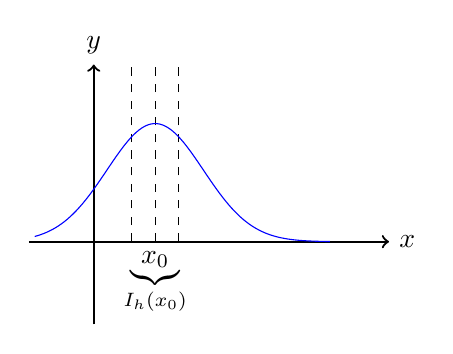
\begin{tikzpicture}[scale=1.5]
        % Axes
        \draw[->,thick] (-0.55,0) -- (2.5,0) node[right] {$x$};
        \draw[->,thick] (0,-0.7) -- (0,1.5) node[above] {$y$};
        % Lines
        \draw[-,dashed] (0.52,0) node[below] {$\underbrace{x_0}_{I_h(x_0)}$} -- (0.52,1.5) node[above] {};
        \draw[-,dashed] (0.72,0) node[below] {} -- (0.72,1.5) node[above] {};
        \draw[-,dashed] (0.32,0) node[below left] {} -- (0.32,1.5) node[above] {};
        % Curve
        \draw[blue,domain=-0.5:2,samples=100] plot (\x, {exp(-3*(\x - 0.52)^2)});
      \end{tikzpicture}        
\end{figure}
We also know that we can approximate the probability by the definition given by the frequentist approach:
\[
    \Pr{X_i \in I_n(X_0)} \approx \frac{\#\{X_i \in I_h(x_0)\}}{n} \approx f_X(x_0) 2 h_n
\]
From this, we can derive that:
\[
    \#\{X_i \in I_h(x_0)\} \approx \underbrace{f_X(x_0) 2}_{const} h_n n \iff \#\{X_i \in I_h(x_0)\} \propto h_n n
\]
From this relation, in order to guarantee the the principle of \textit{locality} we want that for $n \to +\infty$, $h_n \to 0$, while to guarantee \textit{LLN} we need that $h_n n \to +\infty$, which are two reasonable requirements which do not conflict. %TODO: check, non sono siocuro che h_n\cdotn\to\infty sia una condizione che si orienti solo alla LLN

\begin{exercise}
    Assume that $h_n$ scales with law $\frac{1}{n^p}$ with $p>1$. Let us verify the \textit{locality} condition:
    \[
        \lim_{n \to +\infty} h_n = \lim_{n \to +\infty} \frac{1}{n^p} = 0
    \]
    Let us verify the \textit{LLN} condition:
    \[
        \lim_{n \to +\infty} h_n n = \lim_{n \to +\infty} \frac{n}{n^p} = 0 \neq +\infty
    \]
    In this case the naive-kernel estimator is not consistent because we are not satisfying the LLN condition.
\end{exercise}

\begin{exercise}
    Assume $h_n$ scales with law $\frac{1}{\sqrt{n}}$. Let us verify the \textit{locality} condition:
    \[
        \lim_{n \to +\infty} h_n = \frac{1}{\sqrt{n}} = 0
    \]
    Let us verify the \textit{LLN} condition:
    \[
        \lim_{n \to +\infty} h_n n = \lim_{n \to +\infty} \frac{n}{\sqrt{n}} = +\infty
    \]
\end{exercise}

We can conclude that for the naive-kernel estimator, $h_n$ should scale \textbf{sublinearly}.

\paragraph*{Multidimensional case}
If we had $d$ dimensions, since we need to compute the volume of the hypercube that approximates the area under the curve, the number of points would be given by:
\[
    \#\{X_i \in I_h(x_0)\} \approx f_x(x_0) 2 h^d_n n
\]
This means that if we increase $d$, $n$ should grow \textbf{exponentially} to match the growth rate of $h$, and this is also known as the \textit{curse of dimensionality}.

Under that condition, it can be proved that the nearest neighbour estimator is \textbf{weakly consistent}.
\subsubsection{Nearest-neighbour estimator}
For this estimator, the number of points is given by the parameter $k_n$, so the conditions are reversed with respect to the naive estimator.

To guarantee the \textit{LLN} condition, we need that $k_n \to +\infty$, while to guarantee the \textit{locality} condition, we need that $n \to \infty$ because in this way we're increasing the probability that the $k$ chosen points are closer to $x_0$.

By the way, the two conditions are in conflict and we need a condition that allows us to satisfi both requirements. 

We can simply require that:
\[
    \frac{k_n}{n} \to 0
\]
\section{Exercise}
Now we want to implement the theory on non-parametric regression, using the estimators we studied.

Assume we have a random variable $Y$ and a random vector $X \in \mathbb{R}^d$, and we want to estimate the regression function:
\[
    Y = \sin(X) + \mathcal{E}
\]
where $\mathcal{E} \sim N(0,1)$ and $X \sim U(0,a)$.

Let's implement a function that computes the optimal regression function, naive kernel estimator and the nearest neighbour estimator.

Let us now examine the plots.

By selecting $h = 10$ the naive kernel estimator curve has degenerated into a straight line, because the interval is too large with respect to the number of samples, so the estimator just took all of the points and made the average of all the point, that is about zero because the sine is a periodic function. We actually converged to the expectation of $Y$ that is zero.

On the other hand by selecting $k=10$, the nearest neighbour estimator has a shape similar to the one of the sine function.

By selecting $k = 5$ and $h=0.5$, the \textit{naive estimator} starts to take some shape but it is not very similar to the optimal regression function
% i put 10 and 0.1 much better

By changing values, we observed that if $h$ is too small then we will not statisfiy the law of large numbers, and the effect is that...
and if $k$ is too large we lose locality, and the effect is that...

If H is too small i will lose law of large number => 0.01
If K is too larg i will use locality => 50

K = 50 => blue is flattered
H = 0.01 => each point is just the sample, I am enhancing the jumps
-> small H is similar to Knn = 1

if i put K = 100 -> flat line, so i recover large

small k => no LLN
any local avg is not avg but a sample

large K takes all of them but it coverges to the exeception of Y which is close of zero bc we have sin(X)

0.1 and 10

are we statisfied with this learned regression function

we examine what happens with more samples and see if we increase we do better with other number of samples.

1000 of samples
disappointed => blue curve is not nice

Knn =>
if k remains fixed we lose LLN
we are local but the oscillations are great
we are not growing in term of LLN
k must increase with N

recovering LLN

but there are flat => boundary effect because there are not points on the left

increasing K
increasing K

we can acutally converging to the regression function


write this code here and add the analysis of the error
compute the error between these regression function looking at definiction

montecarlo simulation
either with a fixed training set
or
generate a training set each time

for different size of the training set

we need one law that relates k to n or h to n
a
$knn / n \to 0$
$kn \to \infty$
$1/sqrt(N)$

check whether the error is going to zero

check this behaviour of the plot + run simluation
there are not theoretical values


We would expect that the error of the optimal regression function tends to the MMSE, which can be computed as following:
\[
    \text{MMSE} = \E{}{(r(X_0) - Y_0)^2} = \E{}{(\sin(X_0) - \sin(X_0) - \mathcal{E})^2}  = \E{}{\mathcal{E}^2} = 1
\]
